\section{Descripción del problema}

\subsection{Historia de Home Credit}

Home Credit, fundada en 1997 en la República Checa, ha evolucionado desde sus
inicios como un proveedor local de préstamos al consumo hasta convertirse en una
empresa financiera global líder. Desde su fundación, la empresa ha mantenido un
enfoque singular en proporcionar servicios financieros a aquellas poblaciones
que tradicionalmente han tenido un acceso limitado a servicios bancarios. El
modelo de negocio de Home Credit se ha destacado por su capacidad para llegar a
consumidores que no cuentan con historial crediticio o que carecen de acceso a
formas convencionales de financiamiento.

A lo largo de los años, Home Credit ha expandido su presencia a nivel mundial,
estableciendo operaciones en múltiples países de Asia, Europa y América. Su
presencia global le ha permitido adaptarse a diversas realidades económicas y
necesidades financieras locales, consolidándose como una fuerza significativa en
el sector de servicios financieros no bancarios.

La clave del éxito de Home Credit radica en su capacidad para evaluar el riesgo
crediticio de manera innovadora. La empresa ha adoptado tecnologías avanzadas,
como el análisis de datos y el aprendizaje automático, para realizar
evaluaciones precisas de la solvencia crediticia de los clientes. Este enfoque
ha permitido a Home Credit ampliar su alcance a segmentos de la población que a
menudo son pasados por alto por las instituciones financieras tradicionales.

\subsection{Solución a Construir}

En la búsqueda constante de mejorar sus servicios y mantenerse a la vanguardia
de la industria, Home Credit ha identificado la necesidad de optimizar su
sistema de gestión de bases de datos. La solución propuesta para este proyecto
tiene como objetivo abordar los desafíos específicos asociados con la gestión
eficiente de grandes volúmenes de datos y garantizar la integridad y seguridad
de la información.

La implementación de un Sistema de Gestión de Bases de Datos (SGBD) robusto es
esencial para optimizar la normalización y seguridad de la información.
Se busca construir un modelo E-R (Entidad-Relación) que refleje los contenidos de HomeCredit, 
a partir de este modelo se busca construir un modelo relacional que refleje los contenidos 
que serán almacenados en SQL Server.

Para abordar la necesidad de alta disponibilidad y eficiencia en la gestión de
datos, se desarrollará un migrador que permita la hacer una migración de los 
datos almacenados en los archivos CSV a la base de datos. Además, se
implementará un servidor de auditoría para almacenar todo aquel registro que
sea modificado, eliminado o insertado en la base de datos.

La solución incluirá la creación de funciones específicas para la inserción de
datos, asegurando la coherencia y validez de la información introducida en la
base de datos. La aplicación de triggers en todas las tablas garantizará la
verificación de la validez de los valores ingresados, contribuyendo a mantener
la integridad de los datos.

En términos de seguridad, se establecerán diferentes niveles de acceso a través
de la creación de usuarios con permisos específicos, como administrador, usuario
normal y usuario de respaldo. Además, se implementarán índices no clúster para
optimizar el rendimiento de las consultas y consultas SARGABLES que funcionen
como filtros eficientes en un posible sitio web.

La solución propuesta no solo aborda los desafíos técnicos de la gestión de
bases de datos, sino que también se alinea con la misión de Home Credit de
proporcionar servicios financieros eficientes y accesibles a segmentos de la
población que históricamente han enfrentado barreras en este aspecto.

En resumen, la solución a construir se centra en la modernización y optimización
del sistema de gestión de bases de datos de Home Credit, utilizando herramientas
avanzadas para garantizar la eficiencia operativa, la seguridad de la
información y, en última instancia, la capacidad de seguir ofreciendo servicios
financieros innovadores y accesibles a nivel global.

\section{Desarrollo}

\subsection{Modelo E-R}

Para la construcción del modelo E-R se utilizó la herramienta de modelado
\textit{diagrams.net}. El modelo E-R se puede observar en la figura
\ref{fig:er-diagram}.

\begin{figure}[H]
    \centering
    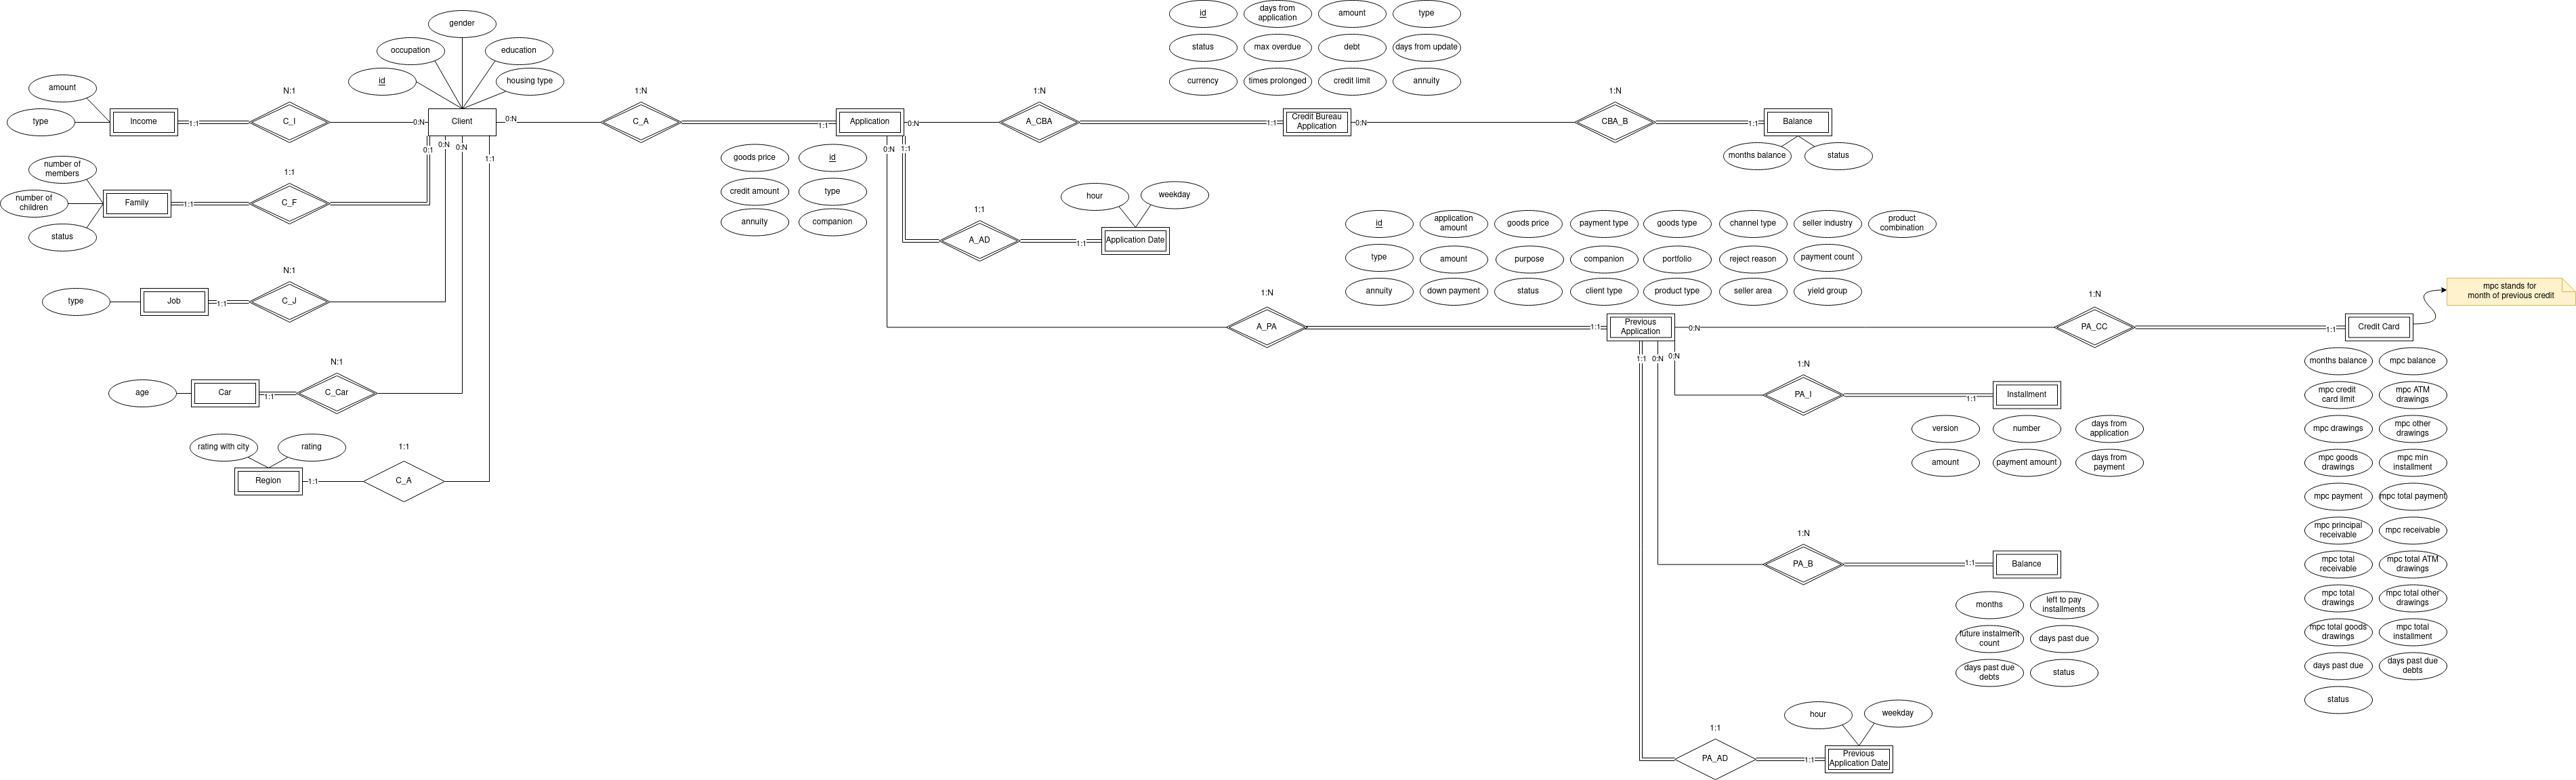
\includegraphics[width=0.8\textwidth]{img/er-diagram.png}
    \caption{Modelo E-R}
    \label{fig:er-diagram}
\end{figure}

\subsection{Modelo Relacional}

El modelor relacional se encuentre basado en el modelo E-R, el cual se puede
observar en la figura \ref{fig:relational-model}. Igualmente desarrollado 
utilizando la herramienta \textit{diagrams.net}.

\begin{figure}[H]
    \centering
    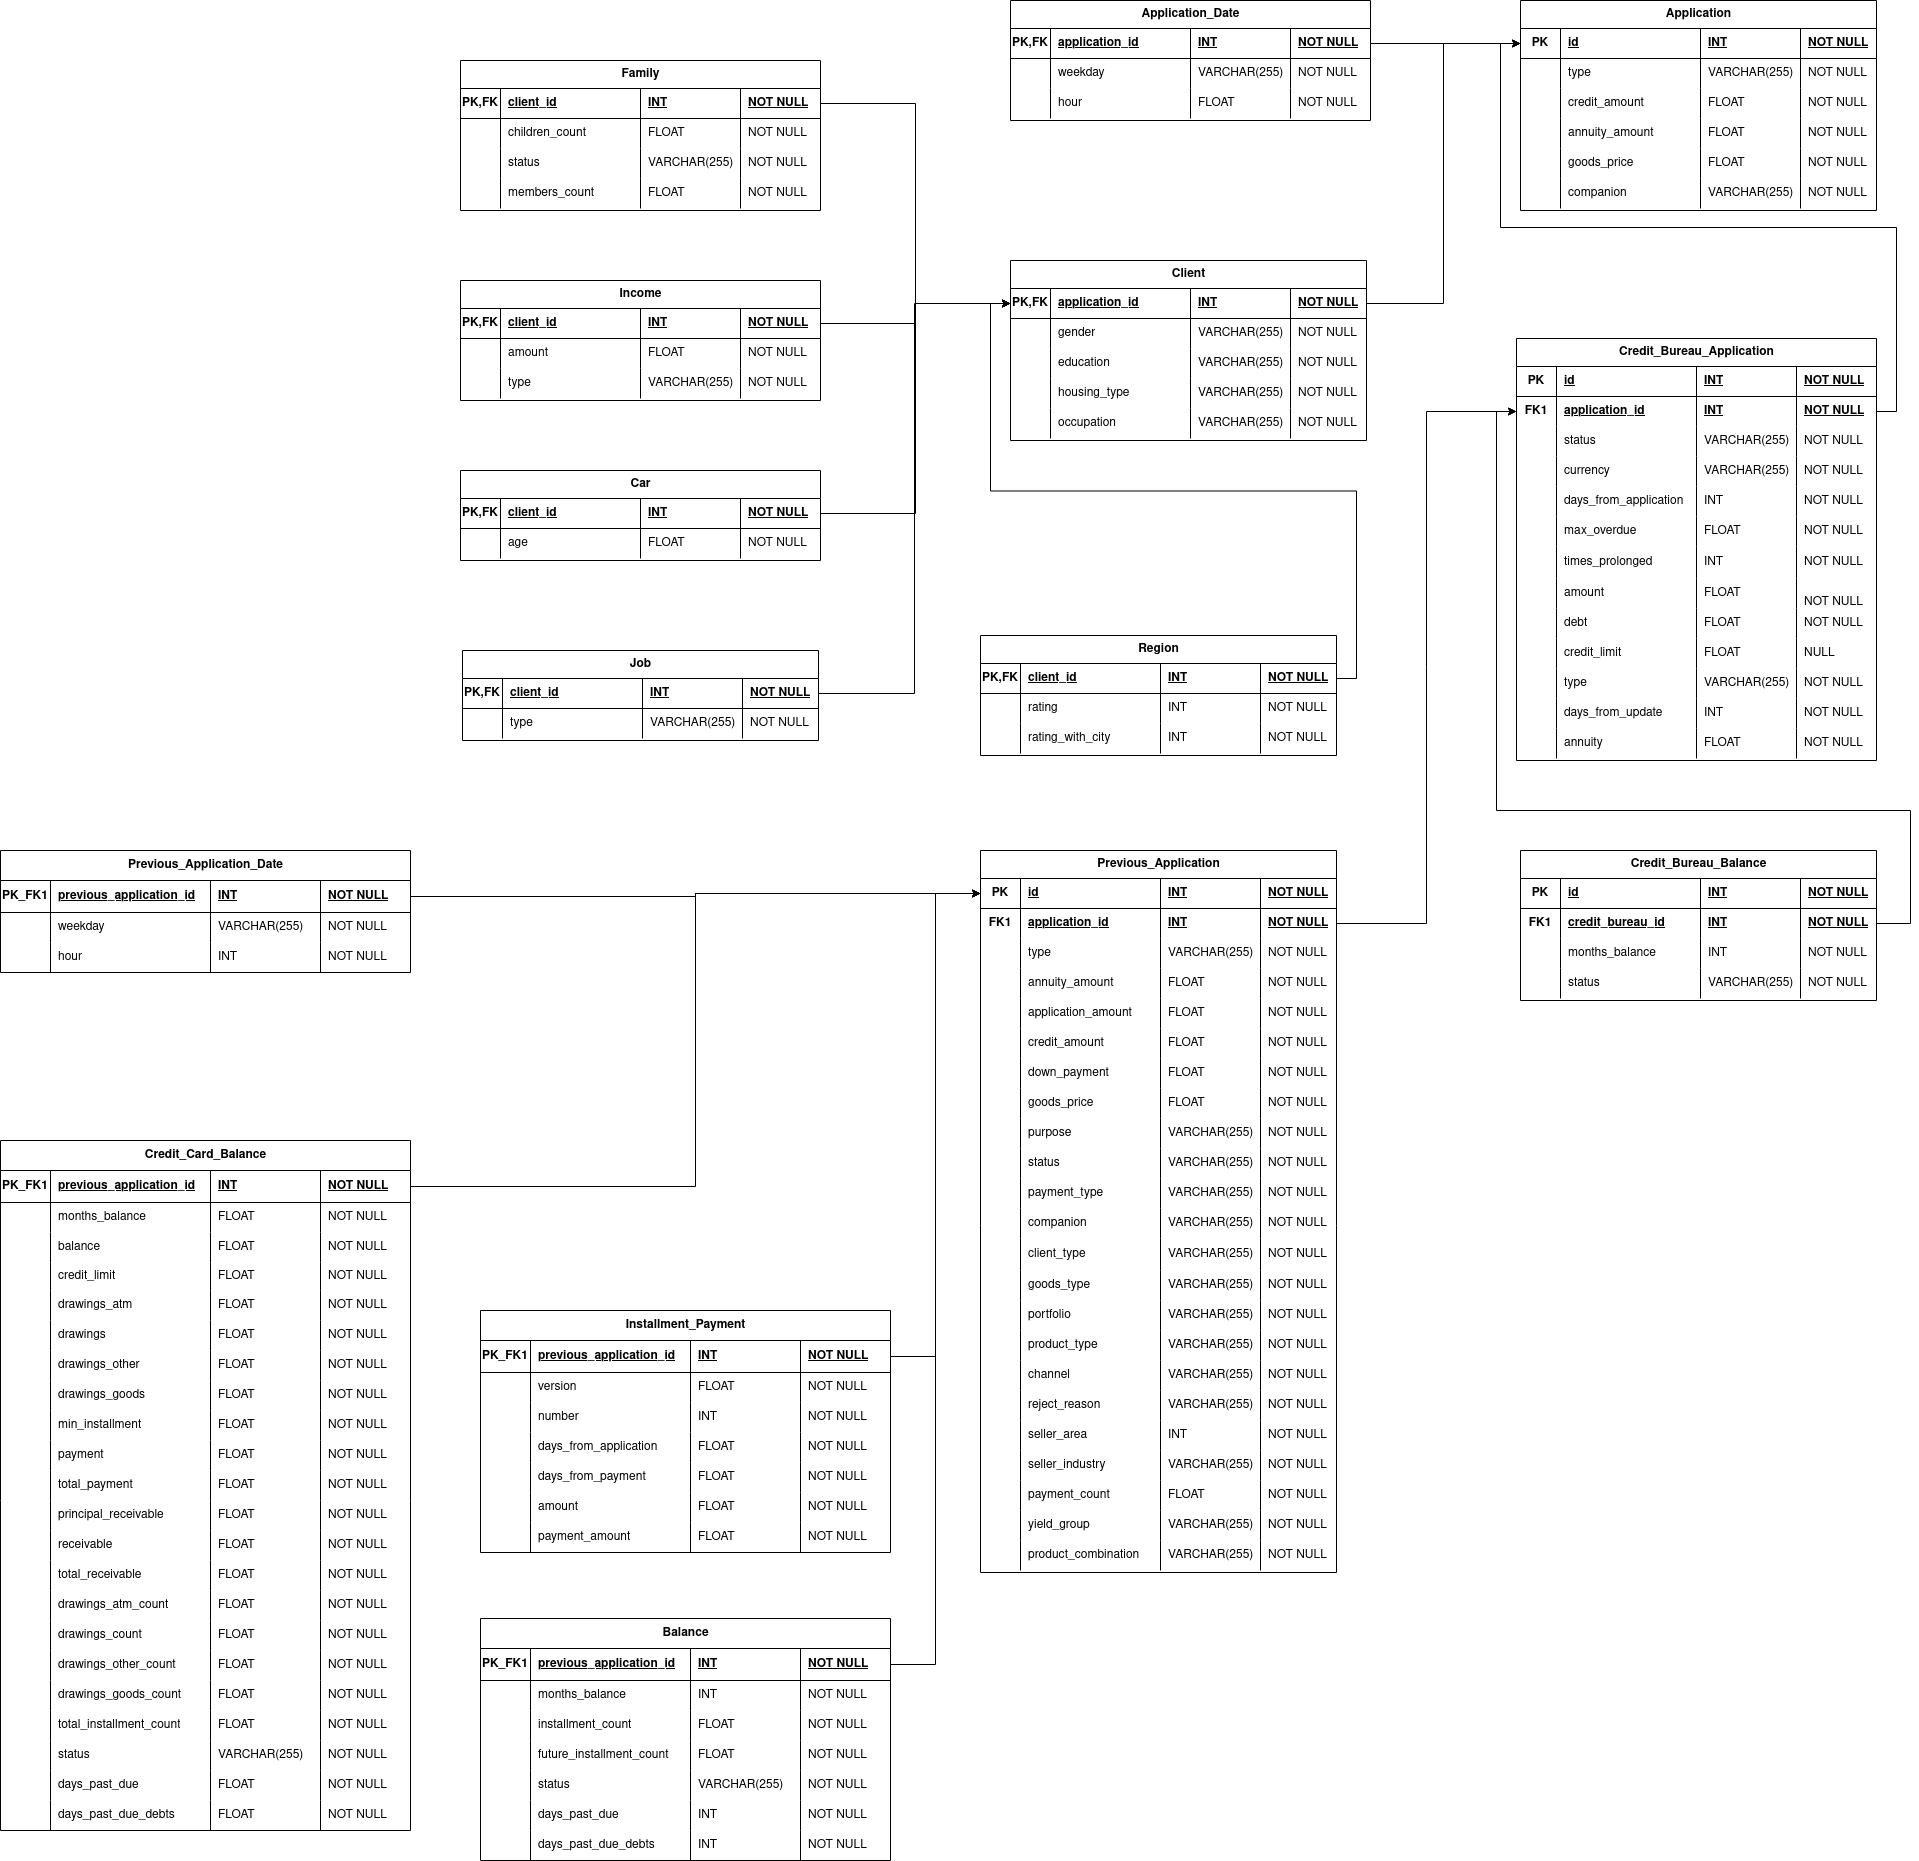
\includegraphics[width=0.6\textwidth]{img/relational-diagram.png}
    \caption{Modelo Relacional}
    \label{fig:relational-model}
\end{figure}

\subsection{Migrador}

Para la construcción del migrador se utilizó el lenguaje de programación Go,
debido a que es un lenguaje de programación compilado, concurrente y de tipo
estático, que tiene como objetivo ser sencillo, eficiente y escalable. La 
principal razón de utilizar este lenguaje de programación es debido a que
ofrece una gran cantidad de librerías en adición a que tiene concurrencia 
nativa, lo cual permite que el proceso de migración sea más rápido.

El migrador utiliza un archivo de configuración en formato JSON, el cual
contiene la información de la base de datos de origen, la base de datos de 
destino y la ruta de los archivos CSV. El migrador se encarga de leer el 
archivo de configuración, conectarse a la base de datos de origen (CSV) y
a la base de datos de destino (SQL Server), para luego realizar la migración
de los datos.

En una computadora con las siguientes características:

\begin{itemize}
    \item Procesador: Intel Core i5-13600K
    \item Memoria RAM: 32 GB 3600 MHz
\end{itemize}

El proceso de migración de los datos tomó aproximadamente 2 horas 
en total, lo cual es un tiempo aceptable para la cantidad de datos que se 
están migrando. Logrando una transmisión de aproximadamente 30,000 registros
por segundo.

\subsection{Servidor de Auditoría}

Para la construcción del servidor de auditoría se utilizó una 
tabla en la base de datos de destino, la cual contiene los siguientes campos:

\begin{itemize}
    \item \textbf{Id:} Identificador único de la auditoría.
    \item \textbf{Fecha:} Fecha en la que se realizó la operación.
    \item \textbf{Usuario:} Usuario que realizó la operación.
    \item \textbf{Tipo:} Tipo de operación que se realizó sobre la tabla.
    \item \textbf{Descripción:} Descripción de la operación que se realizó y 
        en donde se realizó.
\end{itemize}

De esta manera, cada vez que se realice una operación sobre la base de datos 
de destino, se insertará un registro en la tabla de auditoría, el cual 
contendrá la información de la operación que se realizó. Para que esto 
sea posible, se utilizó un trigger en cada tabla de la base de datos de 
destino, el cual se encarga de insertar un registro en la tabla de auditoría 
cada vez que se realice una operación sobre la tabla.

\subsection{Funciones de CRUD}

Para la generación de las funciones de inserción se utilizó el plugin 
\textit{SQL Complete} de \cite{Devart}, el cual permite generar funciones de inserción,
actualización y eliminación de manera automática. El plugin genera las
funciones basado en la tabla que se seleccione, generando una función por cada 
tabla de la base de datos. De esta manera, cada función de CRUD tiene un 
formato regular y se puede utilizar para cualquier tabla de la base de datos.

\subsection{Triggers}

Para la generación de los triggers se estableció un formato regular, el cual 
luego fue enviado a ChatGPT \cite{OpenAI}, una herramienta de inteligencia artificial
que permite generar texto basado en un texto de entrada. De esta manera, se 
generaron los triggers para cada tabla de la base de datos de destino. Cada 
uno de estos triggers hacen validaciones correspondientes a la tabla en la que 
se encuentran, por ejemplo, si se realiza una operación de inserción en la 
tabla de \textit{application\_test}, el trigger se encargará de validar que 
los datos que se están insertando sean válidos, en caso de que no lo sean, 
el trigger no permitirá la inserción de los datos, generando un rollback.

\subsection{Seguridad}

Para la seguridad de la base de datos se crearon tres usuarios, cada uno con 
diferentes permisos. El primer usuario es el usuario de respaldo, el cual 
tiene permisos de lectura y generación de respaldos de la base de datos de
destino. El segundo usuario es el usuario normal, el cual tiene permisos de
lectura y escritura sobre la base de datos de destino, pero no tiene permisos
para realizar modificaciones sobre la estructura de la base de datos. El tercer
usuario es el usuario administrador, el cual tiene permisos de super usuario
sobre la base de datos de destino, lo cual le permite realizar cualquier
operación sobre la base de datos.

\subsection{Índices no Clúster}

Para la creación de los índices no clúster primero se definieron las consultas 
que se realizarían sobre la base de datos, para luego crear los índices no 
clúster basados en estas consultas. De esta manera, las consultas que 
son mostradas en la aplicación web, son consultas que utilizan los índices no 
clúster, lo cual permite que las consultas sean más rápidas y eficientes.

\subsection{Consultas SARGABLES}

Para la creación de las consultas SARGABLES se aprovechan los índices no 
clúster que se crearon anteriormente. De esta manera, las consultas que se 
realizan en la aplicación web son consultas SARGABLES, lo cual permite que 
las consultas sean más rápidas y eficientes, de modo que el usuario pueda
visualizar la información de manera más rápida.

\subsection{Aplicación Web}

Para la construcción de la aplicación web se utilizó el framework de desarrollo 
web \textit{Vue.js} \cite{You}, el cual es un framework progresivo para la creación de 
interfaces de usuario. El framework se encarga de realizar las peticiones a un 
backend, el cual se encuentra desarrollado en el lenguaje de programación Go.

El backend se encarga de realizar las consultas a la base de datos de destino, 
para luego enviar la información a la aplicación web. De esta manera, la 
aplicación web se encarga de mostrar la información de manera ordenada y 
estructurada, para que el usuario pueda visualizar la información de manera 
más sencilla.

Para la visualización de la información se utilizó la librería \textit{Google charts}
\cite{Google}, la cual permite generar gráficos de manera sencilla. De esta manera,
la aplicación web se encarga de generar los gráficos basados en la información 
que se encuentra en la base de datos de destino, para luego mostrarlos al 
usuario en el dashboard de la aplicación web, tal como se puede observar en la 
figura \ref{fig:web-app}.

\begin{figure}[H]
    \centering
    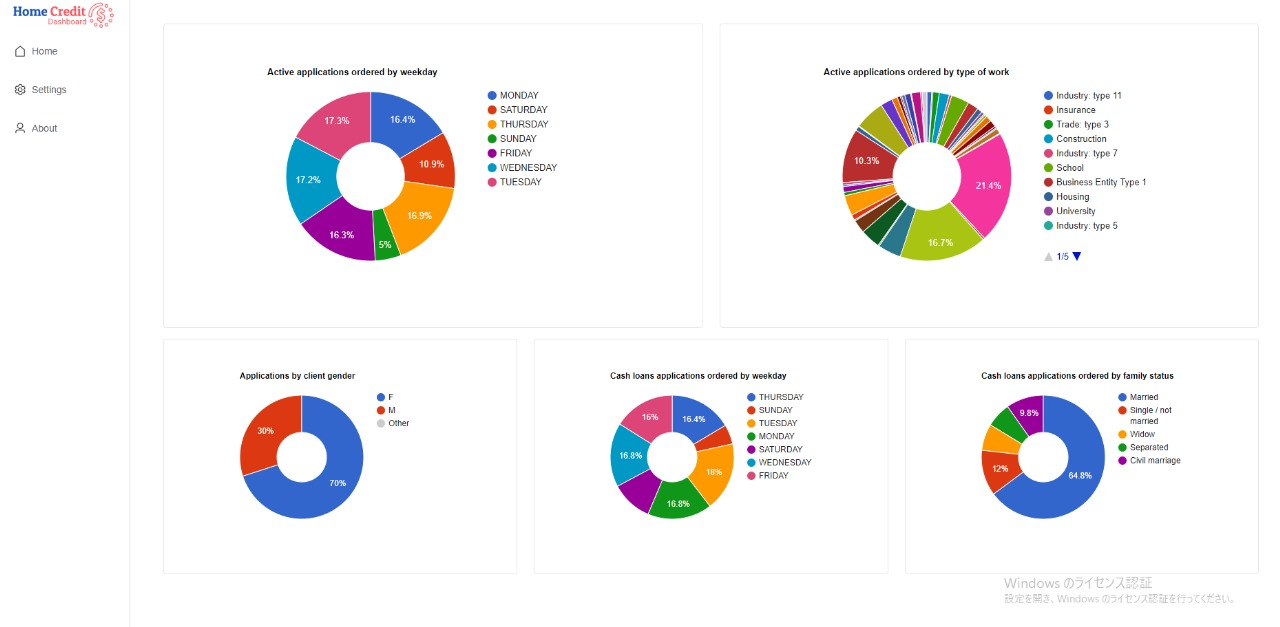
\includegraphics[width=0.8\textwidth]{img/web-app.jpg}
    \caption{Aplicación Web}
    \label{fig:web-app}
\end{figure}
